
%template setup, made it adhere to UWA standards
\documentclass[12pt, a4paper]{article}
\usepackage{graphicx}
\usepackage{amsmath}

%fix caption formatting
\usepackage[font=small,labelfont=bf]{caption}

%slightly modified UWA setup
\setlength{\oddsidemargin}{0.5cm}
\setlength{\evensidemargin}{0.5cm}
\setlength{\topmargin}{-1.6cm}
\setlength{\leftmargin}{0.5cm}
\setlength{\rightmargin}{0.5cm}
\setlength{\textheight}{24.00cm} 
\setlength{\textwidth}{15.00cm}
\parindent 0pt
\parskip 5pt
\pagestyle{plain}


%meta info
\title{Algorithms for RNA folding}
\author{Max Ward \\
School of Computer Science \& Software Engineering \\
The University of Western Australia}
%let the date get auto generated

%author list formatter. not really needed here, but always nice to have
\newcommand{\namelistlabel}[1]{\mbox{#1}\hfil}
\newenvironment{namelist}[1]{%1
\begin{list}{}
    {
        \let\makelabel\namelistlabel
        \settowidth{\labelwidth}{#1}
        \setlength{\leftmargin}{1.1\labelwidth}
    }
  }{%1
\end{list}}



%-------------------------------------------------------------------------

\begin{document}


%title first!
\maketitle

\begin{abstract}
Analysis of thermodynamically based algorithms for RNA structure prediction
\end{abstract}


{\bf Keywords:} Ribonucleic acid, structure, prediction, empirical, comparison.

{\bf CR Classification:} J.3 Biology and genetics.

\clearpage

%\tableofcontents
%\listoffigures
%\clearpage

\section{Introduction}
\subsection{Motivation}
Ribonucleic acid (RNA) is at the core of many biological processes. Traditionally is has been described as the messenger molecule of DNA, faithfully carrying the code for protein from DNA to the site of protein synthesis. However, in a recent landmark paper, Amaral et al. \cite{amaral2008eukaryotic} described our genome, and those of other eukaryotes, as being driven by an RNA machine. They noted that most of the eukaryote genome is transcribed into RNA, despite little of it coding for protein. It seems that much of our genome, originally called `junk DNA', codes for functional RNA molecules. These RNAs can interact with DNA, affecting gene expression. This allows DNA to essentially regulate itself. For example, Makeyev \& Maniati \cite{makeyev2008multilevel} reported that microRNAs affect the expression of genes by interfering with translation of protein. They also argued that microRNAs, and other regulatory RNAs, explain the vast differences between organisms with similar genomes. To put this idea into perspective, we share roughly 90\% of our genes with the domestic Cat \cite{pontius2007initial}. Mattick \cite{mattick2007new} has suggested that the process of development---from embryo to adult---is encoded in the interactions of such RNAs.

A widely held axiom is that chemical structure is tantamount to biological function. With increasingly important biological functions being associated with RNA, it is important to be able to predict its structure. The purpose is this paper is to provide a survey of some widely used RNA structure prediction algorithms. In the interest of keeping this report succinct, I review only algorithms based on a conventional thermodynamically based model. Other algorithms often use machined learned, statistical parameters; these shall not be explored here. In essence, all the algorithms I test take a single RNA primary sequence as input, and return a predicted secondary structure. I hypothesize that newer algorithms should have improved accuracy as compared to older algorithms. In addition, I aim to empirically verify the time complexities of my chosen algorithms. The Zuker algorithm was the first thermodynamic algorithm to achieve usable prediction accuracy, and it forms the basis for all the methods I shall thence discuss.

\subsection{Relevant Algorithms}
\subsubsection{The Zuker Algorithm}
In 1981 Zuker \& Stiegler \cite{zuker1981optimal}
described an algorithm that predicted RNA structure by minimizing molecular free energy. The lower free energy a molecule has, the more stable it is. This was done
by introducing a number of thermodynamic rules for canonical substructures like hairpin loops, internal bulges, multiloops (also called bifurcation loops), unbonded bases, and stacked base pairs. For examples of these structures, refer to Figure \ref{fig:zuk_struct}. The Zuker algorithm uses a mutually recursive dynamic programming recurrence to achieve a relatively comprehensive scoring scheme. This is possible because RNA structures are nested, and hence substructures with minimum free energy need not be recomputed. It follows naturally that dynamic programming can then be used to find a global minimum. The thermodynamic scoring system is borrowed from the work of Studnicka et al. \cite{studnicka1978computer} who presented a
complex but theoretically similar algorithm, albeit having
much worse asymptotic and implementation complexity. It was then later improved by Matthews et al. \cite{mathews1999expanded, mathews2004incorporating}. The time complexity of the Zuker algorithm is $O(n^3)$, where $n$ is the number of nucleotides in the RNA. In short, it is able to efficiently predict secondary structures for RNAs with hundreds of bases, on modern hardware.  Because of
its efficiency, robustness, and extensibility, this method is,
even today, still the most popular available. The most widely used packages for RNA secondary structure prediction all contain implementations of the Zuker algorithm \cite{lorenz2011viennarna, reuter2010rnastructure}.

\begin{figure}
\begin{center}
\scalebox{0.27}{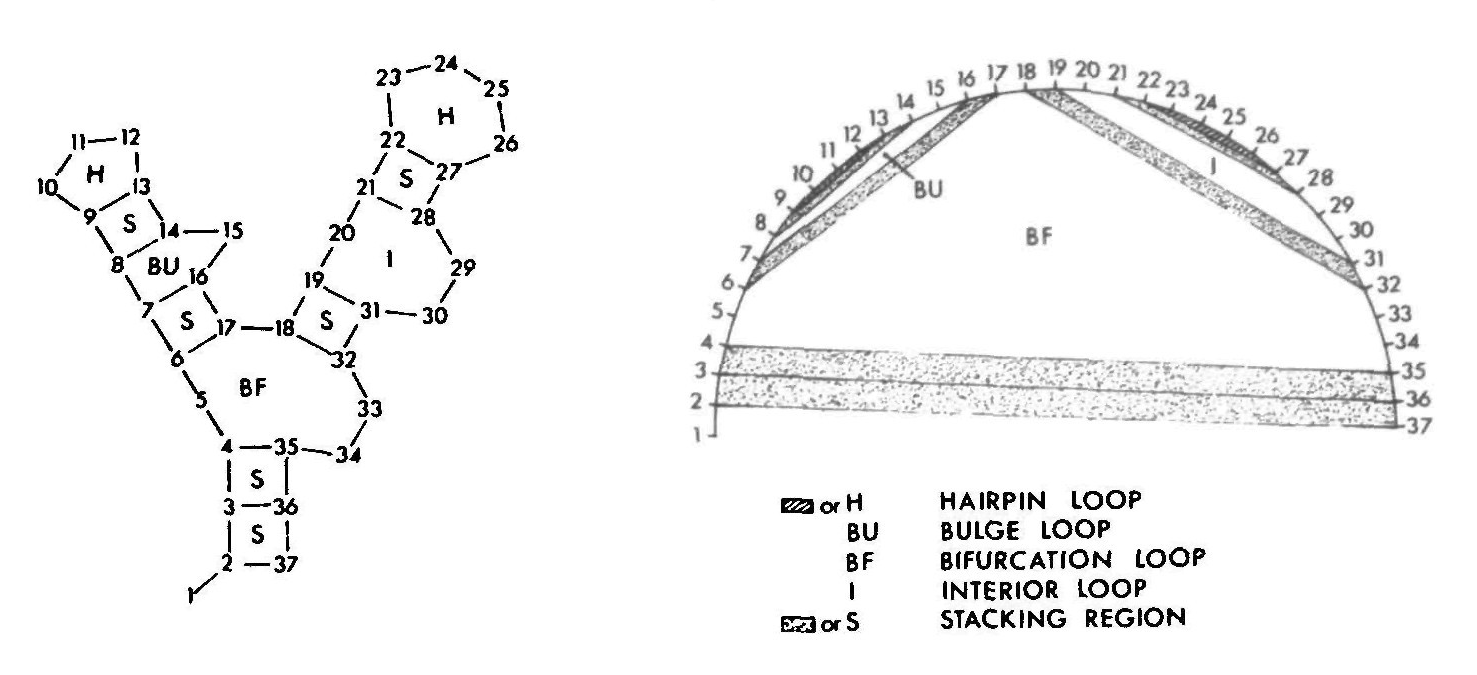
\includegraphics{figure4}}
\end{center}
\caption{Diagram of substructures used in the Zuker algorithm. On the left is a diagram of a RNA secondary structure. On the right is the same structure laid out on a semi-circle. Bonds are represented as lines crossing the semi-circle. Taken from original
publication \cite{zuker1981optimal}.}
\label{fig:zuk_struct}
\end{figure}

\subsubsection{Maximum Expected Accuracy}
The Maximum Expected Accuracy (MEA) technique for RNA prediction was first applied by Do, Woods \& Batzoglou as part of the CONTRAfold algorithm \cite{do2006contrafold} in 2006, and is newer than the Zuker method. The Zuker algorithm essentially finds the most likely structure under a thermodynamic model. A MEA prediction method is more compromising; it finds a structure containing the most probable set of bonds. This is done by computing the partition function for a RNA, as described by McCaskil \cite{mccaskill1990equilibrium}. The partition function computation is achieved by a modified version of the Zuker algorithm, and can be done in $O(n^3)$ time. It should be noted that the this computation uses the underlying thermodynamic model of the Zuker algorithm. This partition function can be processed to produce a two dimensional matrix of base pairing probabilities. Each pair of indexes in the matrix represents the probability that the bases corresponding to those indexes will bond. Intuitively this represents the entire folding landscape of a RNA, rather than a single minimum free energy structure as computed by the Zuker algorithm. A MEA algorithm builds a structure by selecting bonds from this bond probability matrix. However, if the sum probability is naively maximized, it tends to produce structures with too many bonds. As such, a MEA algorithm must find a compromise between the number of bonds selected, and the total probability of the computed structure. Usually this is achieved by introducing some cut-off value, or, in the case of CONTRAfold, a scaling factor.

\subsubsection{Cotranscriptional folding}
Explain in high level terms the three algorithms tested

\section{Materials and Methods}
\subsection{Environment and Software}
All software was run on the Debian 7.5 "wheezy" operating system using the default configuration. Debian was run on top of an Intel i7-4770k processor with 32 gigabytes of RAM. The GNU C Compiler (gcc) version 4.8.2 was used to compile all the required code. Though the processor used was multicore, OpenMP was disabled at compile time to prevent the use of multiple cores during testing. The source code for all the algorithms tested was compiled using makefiles provided as part of their source. The latest version of the Vienna RNA Suite (version 2.1.7, released April 13th 2014) was used as the reference implementation of the MEA algorithm and the Zuker algorithm. The RNAfold module in particular can be used to fold structures using the Zuker algorithm, or to produce a structure with maximum expected accuracy. The entire Vienna RNA Suite was compiled from source, then was linked as a static library at compile time for testing. The latest version of CoFold was downloaded from the CoFold webserver (ref). Because CoFold is based on an older version of RNAfold, it was compiled separately, and linked as a separate static library. In addition, the GNU Regression, Econometrics, and Time-series Library (also called `gretl') was used for all statistical tests, and to produce the graphics found in Section \ref{sec:results}.

\subsection{Data Set}
The RNA secondary structures used to test algorithms presented in this paper were taken from the RNA STRAND database \cite{andronescu2008rna}. The RNA STRAND database is a free-to-use, curated collection of RNA secondary structures taken from various publicly available databases and publications. A subset of RNA structural data was extracted from the database. This subset contained only RNA structures that were marked having been verified using X-Ray crystallography, or nuclear magnetic resonance imaging. It also comprises only whole RNAs; none of the RNAs used were fragments or subsequences of larger RNA molecules. Finally, no duplicates were allowed in the selected set. Hereafter, I shall refer to this collection of RNA secondary structures as the `testing set'. The testing set contained 392 different RNA molecules ranging in length from 20 to 3032 nucleotides.

\subsection{Accuracy}
Well established procedures have been developed over
the history of RNA structure prediction for comparing accuracy. Usually accuracy is determined by comparing predicted structures to known
structures. True Positives ($TP$) is defined as the number of base pairs which appear in both the predicted structure and the actual structure. False Positives
($FP$) is the number of predicted base pairs not in the true
structure \cite{lorenz2011viennarna}. Similarly, False Negatives ($FN$) is defined as the number of base
pairings in the reference structure but not present in the predicted structure \cite{lorenz2011viennarna}.
Sensitivity, also called the True Positive Rate ($TPR$), can be defined using the previously introduced values. I have given a mathematical definition of the $TPR$ in Equation \ref{eq:tpr}.

\begin{equation} \label{eq:tpr}
 \frac{TP}{TP + FN}
\end{equation}

Precision, also known as Positive Predictive Value ($PPV$), can also be calculated
using these values (see Equation \ref{eq:ppv}).


\begin{equation} \label{eq:ppv}
 \frac{TP}{TP + FP}
\end{equation}

For the results presented in this report, the F-score was used as a measure of accuracy. F-score is defined as the harmonic mean of sensitivity and precision. It provides a good balance between these two metrics.

\section{Results}
\label{sec:results}
\subsection{Accuracy}

\begin{figure}
\begin{center}
\scalebox{0.7}{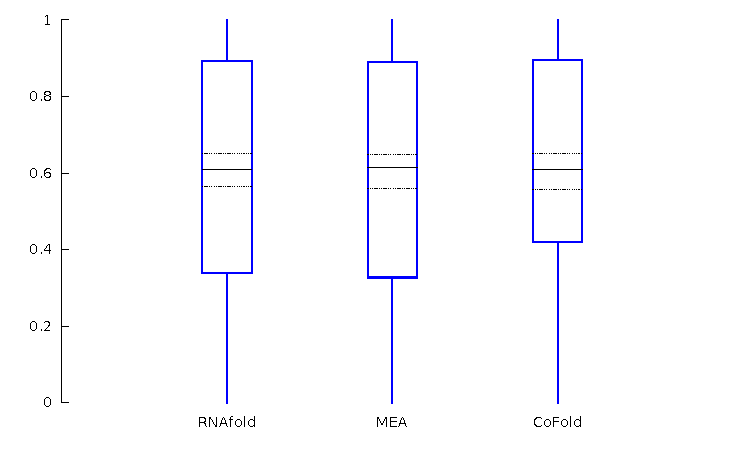
\includegraphics{boxplots}}
\end{center}
\caption{Box plots depicting the spread of F-scores for RNAfold, MEA, and CoFold.}
\label{fig:boxplots}
\end{figure}


\begin{table}
\centering
\begin{tabular}{l*{6}{c}r}
Algorithm	& Mean & Median & Std. Dev. \\
\hline
RNAfold &  0.574834    &    0.608696 & 0.341977   \\
MEA & 0.564584    &    0.615385  & 0.346070\\
CoFold & 0.580802  &     0.608696 & 0.337973  \\
\end{tabular}
\caption{Summary statistics for the F-scores of RNAfold, MEA, and CoFold.}
\label{tab:summarystats}
\end{table}


\begin{table}
\centering
\begin{tabular}{l*{6}{c}r}
Algorithms	& $z$-value & P-value \\
\hline 
MEA \& CoFold &  -0.225675    &    0.410727   \\
RNAfold \& CoFold &  -0.85571    &    0.196079  \\
RNAfold \& MEA &  -0.790628    &    0.214581  \\
\end{tabular}
\caption{The results of Wilcoxon Signed-rank tests between RNAfold, MEA, and CoFold. The $z$-value indicates the magnitude of difference between population F-scores. The P-value indicates statistical significance.}
\label{tab:wilcoxon}
\end{table}


\begin{table}
\centering
\begin{tabular}{l*{6}{c}r}
Algorithms	& $z$-value & P-value \\
\hline 
MEA \& CoFold &  -0.97557    &    0.164639   \\
RNAfold \& CoFold &  -0.284113    &    0.388162  \\
RNAfold \& MEA &  0.290959   &    0.385541  \\
\end{tabular}
\caption{The results of Wilcoxon Signed-rank tests between RNAfold, MEA, and CoFold for only RNA with length $\geq 500$. The $z$-value indicates the magnitude of difference between population F-scores. The P-value indicates statistical significance.}
\label{tab:wilcoxon}
\end{table}


\begin{figure}
\begin{center}
\scalebox{0.8}{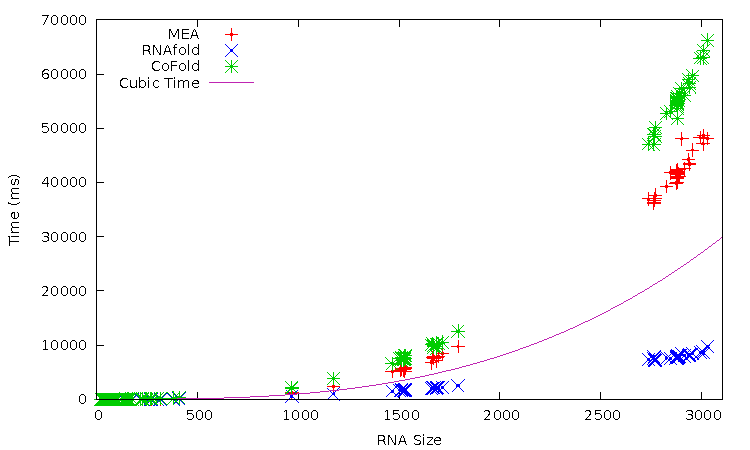
\includegraphics{timegraph}}
\end{center}
\caption{Here the recorded run time for RNAfold, MEA, and CoFold is depicted as a scatter plot. The time used by all algorithms increases with increasing RNA length. The length of an RNA is defined as the number of nucleotides it compromises. A purple line representing a generic cubic curve is included for comparison. This line has been scaled by a constant so that it remains visible on the diagram.}
\label{fig:timegraph}
\end{figure}


\begin{figure}
\begin{center}
\scalebox{0.8}{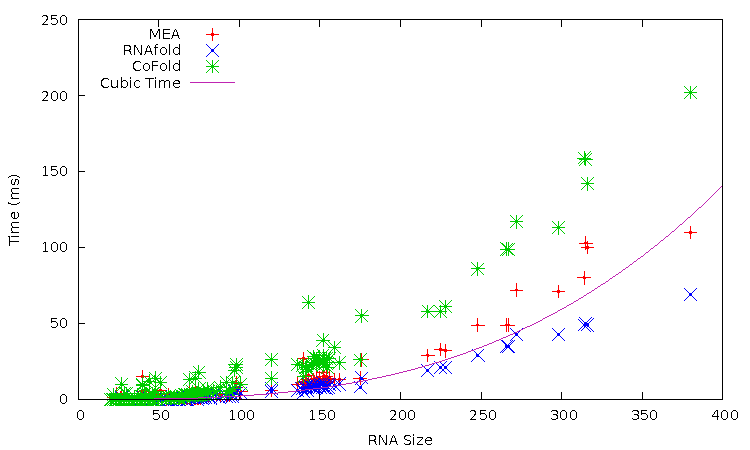
\includegraphics{timegraphsmall}}
\end{center}
\caption{Here the recorded run time for only smaller RNAs ($< 400$ nucleotides) is depicted as a scatter plot. A purple line representing a generic cubic curve is included for comparison. This line has been scaled by a constant so that it remains visible on the diagram.}
\label{fig:timegraphsmall}
\end{figure}







\subsubsection{Small RNA}
\subsubsection{Moderate RNA}
\subsubsection{Large RNA}
\subsection{Time}

\section{Discussion and Conclusions}




%let bibtex do all the hard work
\bibliographystyle{plain}
\bibliography{assignment_two}


\end{document}

